
Comparing the quadratic equations with standard equation,
\begin{align}
    ax^2+2bxy+cy^2+2dx+2ey+f=0\\
    \therefore c=b=0,e=-\frac{1}{2}, a=3,d=\frac{-5}{2},f=2.\\
    \therefore \vec{V}=\myvec{a & b \\ b & c}=\myvec{3 & 0 \\ 0 & 0}\\ \therefore \vec{u}=\myvec{d \\ e}= \myvec{\frac{-5}{2} \\ \frac{-1}{2}}\\ f=2
\end{align}
 Finding the eigen values corresponding to  $\vec{V}$
\begin{align}
    \mid \vec{V}- \lambda \vec{I} \mid =0\\
    \myvec{ 3- \lambda & 0 \\ 0 & -\lambda}=0\\
    \brak{3 - \lambda}\brak{-\lambda}=0 \\
    \therefore \lambda = 0 ,3 
\end{align}
Calculating the eigen vectors corresponding to the $\lambda$ = 0 ,3 respectively,
\begin{align}
    \vec{V}\vec{x}=\lambda\vec{x}\\
    \myvec{3 & 0 \\ 0 & 0}\vec{x}=0 \implies \vec{p_{1}}=\myvec{0 \\1}\\
    \myvec{0 & 0 \\ 0 & -3}\vec{x} = 3\vec{x} \implies \vec{p_{2}}= \myvec{1 \\ 0} \\
\end{align}
Now by eigen decomposition on $\vec{V}$,
\begin{align}
    \vec{V}= \vec{P}\vec{D}\vec{P}^{\top}\\
    where,\vec{P}= \myvec{\vec{p_{1}}&\vec{p_{2}}}\\
    \vec{P}=\myvec{ 0 & 1 \\ 1 & 0}\\
    \vec{D}= \myvec{\lambda_{1} & 0 \\ 0 & \lambda_{2}}\\
    \vec{D}= \myvec{0 & 0 \\ 0 & 3}
\end{align}
Hence equation becomes,
\begin{align}
    \vec{V}= \myvec{ 0 & 1 \\ 1 & 0}\myvec{0 & 0 \\ 0 & 3}\myvec{ 0 & 1 \\ 1 & 0}\\
    \therefore \vec{V}=\myvec{3 & 0 \\ 0 & 0}
\end{align}
To find the vertex of the parabola ,
\begin{align}
    \myvec{\vec{u}^{\top}+ \eta \vec{p_1}^{\top} \\ \vec{V}}\vec{c} = \myvec{-f \\ \eta \vec{p_1}-\vec{u}}\\
    where, \eta = \vec{u}^{\top}\vec{p_1}= \frac{-1}{2}\\
    \implies
    \vec{c}&=\myvec{-\frac{5}{2}& -1 \\ 3 & 0 \\ 0 & 0}\\ \implies \vec{c}& = \myvec{-2 \\ \frac{5}{2}\\ 0}\\ \implies
    \vec{c}&=\myvec{\frac{5}{6} \\\frac{-1}{12}}
\end{align}
\begin{align}
    \because \vec{p_1}^{\top}\vec{c} &= \myvec{0 & 1}\myvec{\frac{5}{6} \\\frac{-1}{12}}\\
    &= \frac{-1}{12}
\end{align}
and,
\begin{align}
    \vec{p_2}^{\top}\vec{V}\vec{p_2}&= \myvec{1 & 0}\myvec{3 & 0 \\ 0 & 0}\myvec{1 \\ 0}\\
    &= 3\\
    \because (\vec{p_1}^{\top}\vec{c}) (\vec{p_2}^{\top}\vec{V}\vec{p_2})&=\frac{-1}{4}<0 
\end{align}
Hence, The given equation has real roots.\\
\begin{figure}[htp]
    \centering
    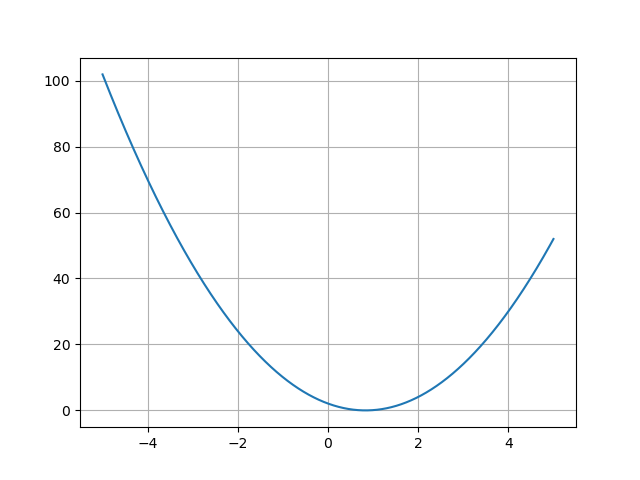
\includegraphics[width=\columnwidth]{solutions/oct/2/21/Figures/Figure_1.png}
    \caption{$3x^2-5x+2$}
\end{figure}
\textbf{ii)}
Comparing the quadratic equations with standard equation,
\begin{align}
    ax^2+&2hxy+by^2+2dx+2ey+f=0\\
    \therefore c&=b,e=\frac{-1}{2}, a=1,d=2,f=5.\\
    \therefore \vec{V}&=\myvec{a & b \\ b & c}=\myvec{1 & 0 \\ 0 & 0}\\ \therefore \vec{u}&=\myvec{d \\ e}= \myvec{2 \\ \frac{-1}{2}}\\ f&=5
\end{align}
Finding the eigen values corresponding to  $\vec{V}$
\begin{align}
    \mid \vec{V}- \lambda \vec{I} \mid &=0\\
    \myvec{ 1- \lambda & 0 \\ 0 & -\lambda}&=0\\
    \brak{1 - \lambda}\brak{-\lambda}&=0 \\
    \therefore \lambda &= 0 ,1 
\end{align}
Calculating the eigen vectors corresponding to the $\lambda$ = 0 ,1 respectively,
\begin{align}
    \vec{V}\vec{x}&=\lambda\vec{x}\\
    \myvec{1 & 0 \\ 0 & 0}\vec{x}&=0 \implies \vec{p_{1}}=\myvec{0 \\1}\\
    \myvec{0 & 0 \\ 0 & -1}\vec{x} &= \vec{x} \implies \vec{p_{2}}= \myvec{1 \\ 0} 
\end{align}
Now by eigen decomposition on $\vec{V}$,
\begin{align}
    \vec{V}&= \vec{P}\vec{D}\vec{P}^{\top}\\
    where,\vec{P}&= \myvec{\vec{p_{1}}&\vec{p_{2}}}\\
    \vec{P}&=\myvec{ 0 & 1 \\ 1 & 0}\\
    \vec{D}&= \myvec{\lambda_{1} & 0 \\ 0 & \lambda_{2}}\\
    \vec{D}&= \myvec{0 & 0 \\ 0 & 1}
\end{align}
Hence equation becomes,
\begin{align}
    \vec{V}&= \myvec{ 0 & 1 \\ 1 & 0}\myvec{0 & 0 \\ 0 & 1}\myvec{ 0 & 1 \\ 1 & 0}\\
    \therefore \vec{V}&=\myvec{1 & 0 \\ 0 & 0}
\end{align}
To find the vertex of the parabola ,
\begin{align}
    \myvec{\vec{u}^{\top}+ \eta \vec{p_1}^{\top} \\ \vec{V}}\vec{c} &= \myvec{-f \\ \eta \vec{p_1}-\vec{u}}\\
    where, \eta &= \vec{u}^{\top}\vec{p_1}\\
    \implies
    \vec{c}&=\myvec{2\\1}
\end{align}
\begin{align}
    \because \vec{p_1}^{\top}\vec{c} &= \myvec{0 & 1}\myvec{2\\1} \\
    &= 1
\end{align}
and,
\begin{align}
    \vec{p_2}^{\top}\vec{V}\vec{p_2}&= \myvec{1 & 0}\myvec{1 & 0 \\ 0 & 0}\myvec{1 \\ 0}\\
    &= 1\\
    \because (\vec{p_1}^{\top}\vec{c}) (\vec{p_2}^{\top}\vec{V}\vec{p_2})=1>0 
\end{align}
Hence, The given equation does not have real roots.\\
\begin{figure}[htp]
    \centering
    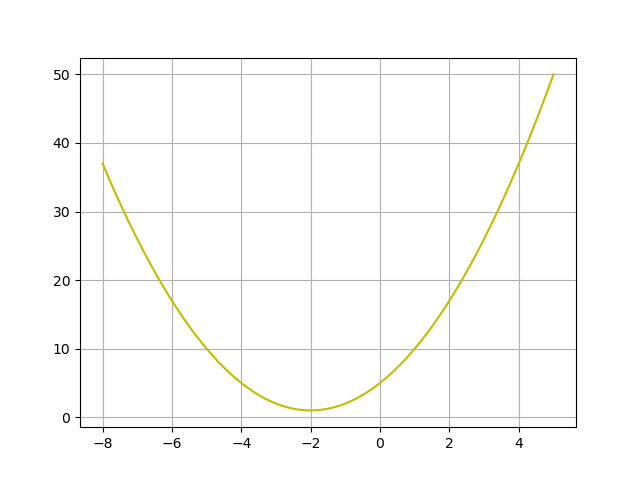
\includegraphics[width=\columnwidth]{solutions/oct/2/21/Figures/Figure_2.png}
    \caption{$x^2+4x+5=0$}
    \label{oct/2/21/fig:my_label}
\end{figure}
\textbf{iii)}
Comparing the quadratic equations with standard equation,
\begin{align}
    ax^2+&2hxy+by^2+2dx+2ey+f=0\\
    \therefore c&=b=0,e=\frac{-1}{2}, a=2,d=-\sqrt{2},f=1.\\
    \therefore \vec{V}&=\myvec{2 & b \\ b & c}=\myvec{1 & 0 \\ 0 & 0}\\ \therefore \vec{u}&=\myvec{d \\ e}= \myvec{-\sqrt{2} \\ -\frac{1}{2}}\\ f&=1
\end{align}
Finding the eigen values corresponding to  $\vec{V}$
\begin{align}
    \mid \vec{V}- \lambda \vec{I} \mid &=0\\
    \myvec{ 2- \lambda & 0 \\ 0 & -\lambda}&=0\\
    \brak{2 - \lambda}\brak{-\lambda}&=0 \\
    \therefore \lambda &= 0 ,2
\end{align}
Calculating the eigen vectors corresponding to the $\lambda$ = 0 ,1 respectively,
\begin{align}
    \vec{V}\vec{x}&=\lambda\vec{x}\\
    \myvec{2 & 0 \\ 0 & 0}\vec{x}&=0 \implies \vec{p_{1}}=\myvec{0 \\1}\\
    \myvec{0 & 0 \\ 0 & -2}\vec{x} &= \vec{x} \implies \vec{p_{2}}= \myvec{1 \\ 0} 
\end{align}
Now by eigen decomposition on $\vec{V}$,
\begin{align}
    \vec{V}&= \vec{P}\vec{D}\vec{P}^{\top}\\
    where,\vec{P}&= \myvec{\vec{p_{1}}&\vec{p_{2}}}\\
    \vec{P}&=\myvec{ 0 & 1 \\ 1 & 0}\\
    \vec{D}&= \myvec{\lambda_{1} & 0 \\ 0 & \lambda_{2}}\\
    \vec{D}&= \myvec{0 & 0 \\ 0 & 2}
\end{align}
Hence equation becomes,
\begin{align}
    \vec{V}&= \myvec{ 0 & 1 \\ 1 & 0}\myvec{0 & 0 \\ 0 & 2}\myvec{ 0 & 1 \\ 1 & 0}\\
    \therefore \vec{V}&=\myvec{2 & 0 \\ 0 & 0}
\end{align}
To find the vertex of the parabola ,
\begin{align}
    \myvec{\vec{u}^{\top}+ \eta \vec{p_1}^{\top} \\ \vec{V}}\vec{c} &= \myvec{-f \\ \eta \vec{p_1}-\vec{u}}\\
    where, \eta &= \vec{u}^{\top}\vec{p_1}\\
    \implies
    \vec{c}&=\myvec{\frac{1}{\sqrt{2}}\\0}
\end{align}
\begin{align}
    \because \vec{p_1}^{\top}\vec{c} &= \myvec{0 & 1}\myvec{\frac{1}{\sqrt{2}}\\0} \\
    &= 0
\end{align}
and,
\begin{align}
    \vec{p_2}^{\top}\vec{V}\vec{p_2}&= \myvec{1 & 0}\myvec{1 & 0 \\ 0 & 0}\myvec{1 \\ 0}\\
    &= 1\\
    \because (\vec{p_1}^{\top}\vec{c}) (\vec{p_2}^{\top}\vec{V}\vec{p_2})=0=0 
\end{align}
Hence, The given equation has equal real roots.
\begin{figure}[htp]
    \centering
    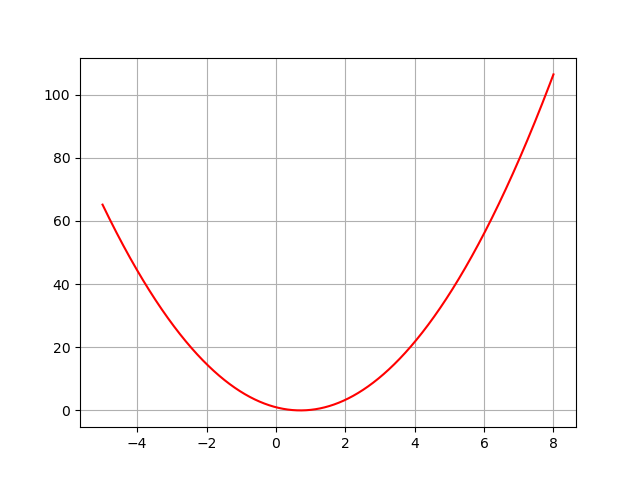
\includegraphics[width=\columnwidth]{solutions/oct/2/21/Figures/Figure_3.png}
    \caption{$2x^2-2\sqrt{2}x+1=0$}
    \label{oct/2/21/fig}
\end{figure}\\
% \cleardoublepage 
% \textbf{Our results:}\\\\
% \begin{tabular}{ |p{2.5cm}||p{1.5cm}|p{1.5cm}|p{1.5cm}|p{1cm}|p{1cm}|p{1cm}| p{2.5cm}|p{2cm}| }
%  \hline
%  Equation & $\vec{V}$ & $\vec{D}$ &$\vec{P}$&$\eta$ & $\vec{c}$& $\vec{p_1}$ & $(\vec{p_1}^{\top}\vec{c}) (\vec{p_2}^{\top}\vec{V}\vec{p_2})$& result \\
%  \hline
%  $3x^2-5x+2=0$   & $\myvec{3 & 0 \\ 0 & 0}$    & $\myvec{0 & 0 \\ 0 & -3}$ & $\myvec{ 0 & 1 \\ 1 & 0} $ & $\frac{-1}{2}$ & $\myvec{\frac{5}{6} \\\frac{-1}{12}}$&$\myvec{0 \\ 1}$ & $<0$& Has real roots  \\
%  $x^2+4x+5=0$ &   $\myvec{1 & 0 \\ 0 & 0}$    & $\myvec{0 & 0 \\ 0 & 1}$   &$\myvec{ 0 & 1 \\ 1 & 0} $ & $\frac{-1}{2}$ & $\myvec{2 \\ 1}$ &$\myvec{0 \\ 1}$& $>0$ & Has no real roots\\
%  $2x^2-2\sqrt{2}x+1=0$ &$\myvec{2 & 0 \\ 0 & 0}$& $\myvec{0 & 0 \\ 0 & 2}$    &$\myvec{ 0 & 1 \\ 1 & 0} $ & $\frac{-1}{2}$  & $\myvec{\frac{1}{\sqrt{2}} \\ 0}$& $\myvec{0 \\ 1}$& =0 & Has equal roots\\

%  \hline
% \end{tabular}
